\chapter{Experimente und Ergebnisse}
In diesem Kapitel werden verschiedene Experimente mit dem FPGA durchgeführt. Zunächst wird gemessen, Wie viel Zeit pro trainiertem Perzeptron für das Training und die Voraussagen auf dem FPGA und einer Implementierung auf dem Hostsystem aufgewendet werden muss. Hierbei wird das Programm auf dem Hostsystem nicht parallelisiert. 
Dann werden beispielhaft Trainingsvorgänge mit verschiedenen Datensätzen durchgeführt, um die Genauigkeit der Vorhersagen zu überprüfen und Ergebnisse der Testvorgänge zu präsentieren.\\
Es werden für die Experimente die Datensätze MNIST \cite{MNIST}, und verwendet.\\
Die Features $\vec f$ des jeweiligen Datensatzes wurden normalisiert, so dass $\forall f \in \vec f\text{ . } f \in [0,1]$. 
\section{Regularisierung}
Mit dem MNIST Datensatz wurden verschiedene Testzyklen zur Regularisierung durchgeführt. Für die Ergebnisse ist der Datentyp, soweit nicht anders vermerkt, auf eine Fixkommazahl mit einem Vorzeichen-, 4 Vorkommastellen- und 11 Nachkommastellenbits eingestellt. Ein Trainingsdurchlauf mit 200 Variablen und 100 Wiederholungen führte zu folgenden Ergebnissen: \\\\
\begin{tabularx}{\textwidth}{p{0.16\textwidth}|r|r|r|r|r}
Perceptron & Regularisierungsrate & Lernrate & Batch & Methode & Genauigkeit\\
\hline
a & 0.0 & 0.100098 & 1 & keine & 95.43\%\\
\hline
b & 0.007812 & 0.100098 & 1 & L2 & 95.75\%\\
\hline
c & 0.009766 & 0.100098 & 1 & L2 & 95.75\%\\
\hline
d & 0.5 & 0.100098 & 1 & L2 & 89.9\%\\
\hline
e & 0 & 0.100098 & 1 & L1 & 95.43\%\\
\hline
f & 0.000977 & 0.100098 & 1 & L1 & 95.43\%\\
\hline
g & 0.004883 & 0.100098 & 1 & L1 & 94.38\%\\
\hline
h & 0.009766 & 0.100098 & 1 & L1 & 93.38\%\\
\end{tabularx}\\\\
Hierbei wurde der Datensatz so angepasst, dass alle Variablen die die Ziffer "`3"' darstellen mit "`trifft zu"' und alle anderen Variablen mit "`trifft nicht zu"' markiert wurden.\\
Nach dem Auswerten der Koeffizienten sind die Einflüsse der Regularisierungsmethoden auf das gelernte Modell deutlich sichtbar. Die Ridge Regression erzielte bei diesem Versuch die besten Ergebnisse, was aufgrund der Daten nicht besonders überraschend war. Da MNIST aus 28x28 Pixeln in Schwarz-Weiß Werten besteht und diese eine handgeschriebene Ziffer repräsentieren war anzunehmen dass es nur wenige Features gibt  welche für das Ergebnis irrelevante Ausprägungen bieten. Demnach ist die LASSO Methode für diesen Datensatz nicht gut geeignet. Die Ridge Regression kann, mit ausreichend kleinem $C$, die Koeffizienten, die zu starke Auswirkungen auf das Modell haben reduzieren, sodass einem Overfitting entgegengewirkt wird. Allerdings hat der gewonnene Genauigkeitswert nur geringfügig zugenommen.\\
Zeichnet man die Koeffizienten als Graphen auf kann man die Auswirkung der Regularisierung auf die Regression deutlich erkennen. In den nachfolgenden Abbildungen 5.1, 5.2 und 5.3 werden diese Graphen dargestellt. Die Koeffizienten sind hierbei die Ergebnisse der obigen Trainingsdurchlaufs.
\begin{figure}[ht]
\centering
  	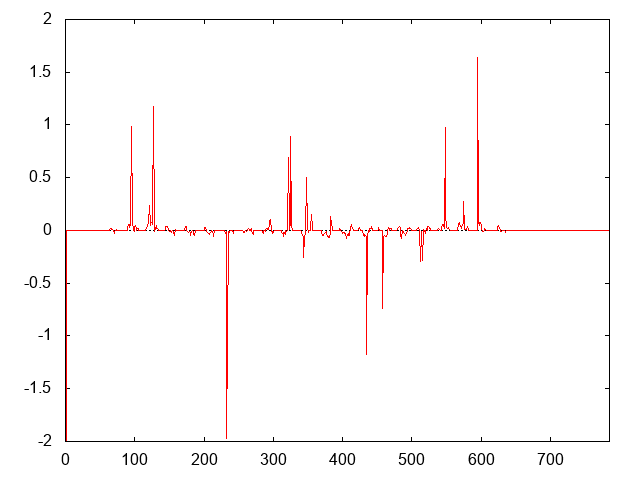
\includegraphics[scale=0.5]{bilder/features7}
  	\caption{L1 Regularisierung}
\end{figure}
\begin{figure}[ht]
\centering
  	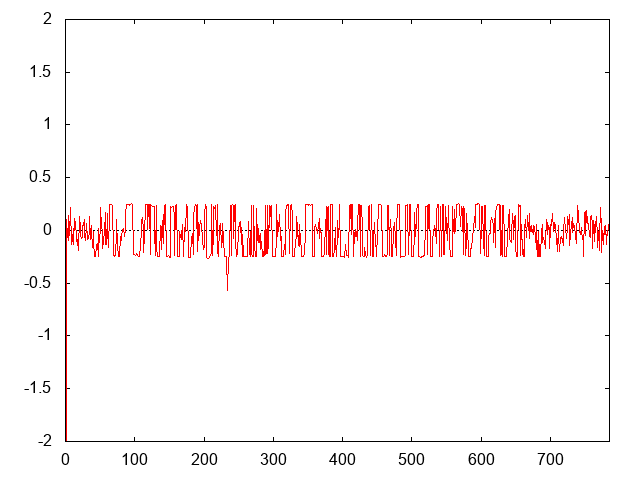
\includegraphics[scale=0.5]{bilder/features2}
	\caption{L2 Regularisierung}
\end{figure}
\begin{figure}[ht]
\centering
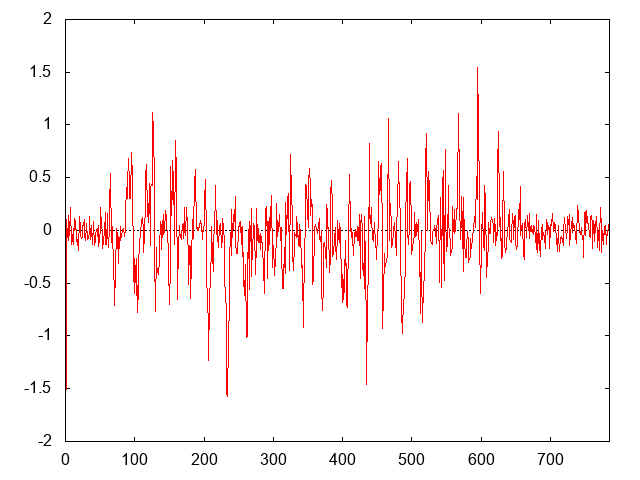
\includegraphics[scale=.5]{bilder/features0}
\caption{Logistische Regression ohne Regularisierung}
\end{figure}\newpage
Bei der Verarbeitung von Bilddaten gibt es den großen Vorteil, dass sich die Koeffizienten selbst als Bild interpretieren lassen. In der ersten Zeile der folgenden Grafiken (Abbildung 5.4, 5.5, 5.6) wurden die Koeffizienten unverändert interpretiert, sodass negative Werte keinen Farbunterschied hervorrufen. Es sind auf den Bildern nur die Koeffizienten zu sehen die einen positiven Einfluss auf die Ausgabe haben, da sie die Features repräsentieren die das Vorhandensein einer Linie belohnen. Der Verlauf ist von Schwarz (keine oder negative Auswirkung) bis hin zu Weiß (positive Auswirkung).\\
In der zweiten Zeile (Abbildung 5.7, 5.8, 5.9) sind die Koeffizienten normalisiert worden, sodass die kleinste Ausprägung 0 und die größte Ausprägung 1 darstellen. Es wird also auch der negative Einfluss der Features berücksichtigt, also derer, die das Vorhandensein einer Linie bestrafen.\newpage
\begin{figure}[ht]
\centering
	\begin{minipage}[b]{.25\linewidth}
  		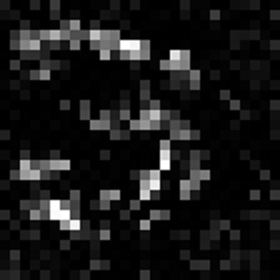
\includegraphics[scale=0.7]{bilder/l0_3}
  		\caption{ohne Regularisierung}
  	\end{minipage}
  	\hspace{.05\linewidth}% Abstand zwischen Bilder
  	\begin{minipage}[b]{.25\linewidth}
  		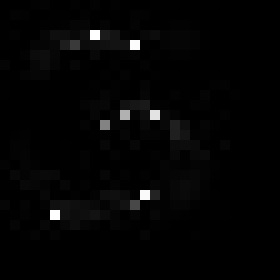
\includegraphics[scale=0.7]{bilder/l1_3}
		\caption{L1 \\Regularisierung}
	\end{minipage}
	\hspace{.05\linewidth}% Abstand zwischen Bilder
	\begin{minipage}[b]{.25\linewidth}
  		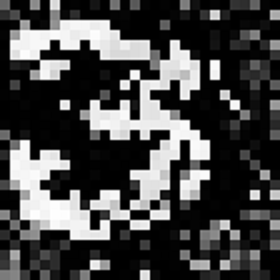
\includegraphics[scale=0.7]{bilder/l2_3}
  		\caption{L2 \\ Regularisierung}
  	\end{minipage}
	\begin{minipage}[b]{.25\linewidth}
  		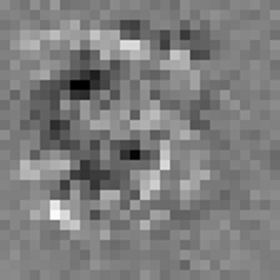
\includegraphics[scale=0.7]{bilder/l0_3_g}
  		\caption{ohne Reg. normiert}
  	\end{minipage}
  	\hspace{.05\linewidth}% Abstand zwischen Bilder
  	\begin{minipage}[b]{.25\linewidth}
  		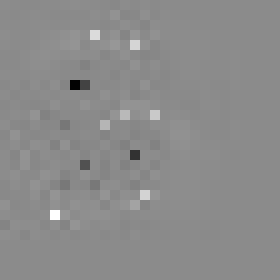
\includegraphics[scale=0.7]{bilder/l1_3_g}
		\caption{L1 normiert}
	\end{minipage}
	\hspace{.05\linewidth}% Abstand zwischen Bilder
	\begin{minipage}[b]{.25\linewidth}
  		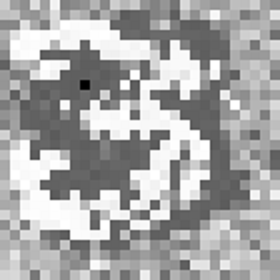
\includegraphics[scale=0.7]{bilder/l2_3_g}
  		\caption{L2 normiert}
  	\end{minipage}
\end{figure}
3